%-------------------------------------------------------------------------------
%   LATEX SOURCE FILE
%-------------------------------------------------------------------------------
\documentclass[twocolumn,letterpaper,10pt,twoside]{jwreport}
%
% The class jwreport is a copy of report.cls, altered so that chapters,
% sections etc appear in SS font
%
%   Packages
\usepackage{multirow}
\usepackage{graphicx}
\usepackage{fancyhdr}
\usepackage{amsmath}
\usepackage{epsfig}
\usepackage{lscape}
\usepackage{rotating}
\usepackage{datetime}
\usepackage{natbib}
\usepackage{times}
\usepackage{epsfig}
\usepackage[ansinew]{inputenc}
%\usepackage{psfrag}
\usepackage{amsfonts}
\usepackage{amssymb}
\usepackage{subfigure}
\usepackage[active]{srcltx}  %SRC Specials for inverse DVI search
% references by chapter
\usepackage{chapterbib}
% use include{chapter} instead input{chapter.tex}
\usepackage{float} % place figure h!
\usepackage{cancel} %
%\usepackage[dvipdfm]{hyperref} % introducing cross reference in labels.
\usepackage{hyperref} % introducing cross reference in labels.
\usepackage{epstopdf}
\renewenvironment{enumerate}%
  {\begin{list}{\arabic{enumi}.}%
     {\topsep=0in\itemsep=0in\parsep=0in\partopsep=0in\usecounter{enumi}}%
   }{\end{list}}
\usepackage{url}

%  Page layout options
\pagestyle{fancy}
%  Margins
\pdfpagewidth 8.5in
\pdfpageheight 11in
\setlength\topmargin{-.55in} % original size -.55
\setlength\headheight{0.5in}
\setlength\headsep{0.5in}
\setlength\textheight{8.8in}
\setlength\textwidth{6.5in}
\headwidth=6.5in
\setlength\oddsidemargin{0.1in}
\setlength\evensidemargin{-.1in}
\setlength\headheight{40pt}
\setlength\headsep{0.5in}

\parindent=0.0in

\font\ninerm=cmr9
\font\tenrm=cmr10
\font\sevrm=cmr7
% Set up sans-serif etc
\renewcommand{\footrulewidth}{0.0pt}
\renewcommand{\headrulewidth}{0.0pt}
\renewcommand{\chaptermark}[1]{%
\markboth{\MakeUppercase{%
\chaptername}\ \thechapter:%
\normalfont\normalsize\sffamily\slshape\ #1}{}}
\lhead{}
\rhead{}
\lfoot{}
\cfoot{\sf \fancyplain{\thepage}{\thepage}}
%\rfoot{Draft version: \ampmtime~\ddmmyyyydate \today}
\rfoot{}
\chead{}
% Set up referencing
\bibpunct{(}{)}{;}{a}{,}{;}
\renewcommand\bibname{References}
\renewcommand\bibsection{\section{\refname}} % make references a section*

% set up equation/figure numbering
\setcounter{secnumdepth}{3} % number untill subsubsection!!!
%%
%\renewcommand{\thechapter}{\Roman{chapter}}
%\renewcommand{\theequation}{\thesection.\arabic{equation}}
\renewcommand{\thetable}{\arabic{table}}
\renewcommand{\thefigure}{\arabic{figure}}
%%
%\usepackage{pdfpages}  % full cover page
% Extra hyphenation list
\hyphenation{aniso-tropy aniso-tropic micro-seismic}

%-------------------------------------------------------------------------------
%   Definitions                     % set report year and volume
%-------------------------------------------------------------------------------
\newcommand{\thereportyear}{2016} % used in all Chapters
\newcommand{\thereportvolume}{7}

%-------------------------------------------------------------------------------
%   Document body
%-------------------------------------------------------------------------------
\begin{document}
%
%
\baselineskip=20pt
%
%-----------------------------------------------------------------------
%   TITLE PAGE
%-----------------------------------------------------------------------
%
%\includepdf{2013cover.pdf}
\newpage\thispagestyle{empty}
\cleardoublepage
\begin{titlepage}
\begin{center}

\begin{figure}
\centering
  % Requires \usepackage{graphicx}
  \includegraphics*[width=3cm]{logo.jpg}
\end{figure}

%\baselineskip=30pt

\setlength{\unitlength}{1in}
\begin{picture}(6,0.1)
\thicklines
\put(0,0.05){\line(6,0){6}}
\put(0,0.0){\line(6,0){6}}
\end{picture}

\baselineskip=12pt
\vspace*{0.3in}
{\huge \bf \sf MICROSEISMIC INDUSTRY CONSORTIUM\\~\\ }
{\huge  \bf \sf Annual Research Report: Volume \thereportvolume\ -- \thereportyear}
\vspace*{0.3in}

\begin{picture}(6,0.0)
\put(0,0.05){\line(6,0){6}}
\put(0,0){\line(6,0){6}}
\end{picture}

\vspace{1in}
\begin{large}
{\bf University of Alberta}\\~\\
{\em Department of Physics \\
Edmonton, Alberta\\
Canada}
\end{large}

%\vspace{0.1in}

\vspace{.5cm}
and
\vspace{0.5cm}

\begin{large}
{\bf University of Calgary}\\~\\
{\em
Department of Geoscience\\
Calgary, Alberta\\
Canada}
\end{large}

\vspace{0.2in}

%\vspace{4.0cm}
%{\large \bf \sf http://earth.leeds.ac.uk/bliss} \\

\vspace{0.5in}

%\today

{\bf \sf November, \thereportyear}
\vspace{0.5in}


\begin{picture}(6,0.0)
\put(0,0.05){\line(6,0){6}}
\put(0,0){\line(6,0){6}}
\end{picture}


\end{center}
\end{titlepage}

\newpage\thispagestyle{empty}
~\\
%\cleardoublepage
%----------------------------
%  PREAMPLE
%----------------------------
\pagenumbering{roman}
\setcounter{page}{0}
%\chapter*{Acknowledgments}\label{chap:ackn}
\addcontentsline{toc}{chapter}{Acknowledgements}
The Microseismic Industry Consortium gratefully acknowledges the support of the
following organizations and companies:
\vspace{0.5in}


\begin{figure}[htb]
  % Requires \usepackage{graphicx}
  \includegraphics*[width=2cm]{sponsors/anadarko}
  \includegraphics*[width=2cm]{sponsors/apache}
  \includegraphics*[width=2.5cm]{sponsors/arcResources}
  \includegraphics*[width=2cm]{sponsors/birchcliff}
   \includegraphics*[width=2cm]{sponsors/cameco}
    \includegraphics*[width=2cm]{sponsors/canadianNaturalResources}
     \includegraphics*[width=2cm]{sponsors/cggVeritas}
     \includegraphics*[width=2cm]{sponsors/chevron.jpg}
      \includegraphics*[width=2cm]{sponsors/conocoPhillips}
       \includegraphics*[width=2cm]{sponsors/encana}
        \includegraphics*[width=2cm]{sponsors/eogResources}
         \includegraphics*[width=2cm]{sponsors/esgSolutions}
          \includegraphics*[width=2cm]{sponsors/hess}
           \includegraphics*[width=2cm]{sponsors/huskyEnergy}
            \includegraphics*[width=2cm]{sponsors/ion}
             \includegraphics*[width=2cm]{sponsors/itasca}
              \includegraphics*[width=2cm]{sponsors/microseismic}
               \includegraphics*[width=2cm]{sponsors/nanometrics}
                \includegraphics*[width=2cm]{sponsors/nexen}
                 \includegraphics*[width=2cm]{sponsors/noble-energy-logo}
                  \includegraphics*[width=2cm]{sponsors/pennwestEnergy}
                   \includegraphics*[width=2cm]{sponsors/petroBras}
                    \includegraphics*[width=2cm]{sponsors/pinnacle}
   \includegraphics*[width=2cm]{sponsors/pioneer}
   \includegraphics*[width=2cm]{sponsors/pot_logo}
   \includegraphics*[width=2cm]{sponsors/schlumberger}
   \includegraphics*[width=2cm]{sponsors/shell}
   \includegraphics*[width=2cm]{sponsors/spectraseis}
   \includegraphics*[width=2cm]{sponsors/talismanEnergy}
   \includegraphics*[width=2cm]{sponsors/transform}
   \includegraphics*[width=2cm]{sponsors/trican}\\
   \begin{center}
   \includegraphics*[width=3cm]{sponsors/nserc_logo}
   \end{center}

\end{figure}


%\begin{Large}
%\begin{center}
%\begin{bf}
%Chevron\\
%%Shell\\
%StatoilHydro
%~\\
%ITF \\
%\end{bf}
%\end{center}
%\end{Large}
%
\vspace{0.5in}

%-------------------------------------------------------------------------------
%\begin{figure*}[ht]
%\centering
%\epsfig{file=SPONSORS/lump_logos.eps,width=0.9\linewidth}
%\end{figure*}
%-------------------------------------------------------------------------------
 % inclde sponsors page with logos final compilation
%\cleardoublepage
%
\tableofcontents
\cleardoublepage
%-----------------------------------------------------------------------
%   CHAPTERS
%-----------------------------------------------------------------------
\baselineskip=12pt % 12 pts line spacing in 2014 template
\parindent = 18pt
%
\setcounter{page}{0}
\pagenumbering{arabic}%
%\chapter*{Preface}
\addcontentsline{toc}{chapter}{Preface}
%
%\section*{Introduction and motivation}
%
Microseismic techniques have emerged as an important approach for {\em in situ} monitoring of fracture processes, whether for hydrofrac stimulation of tight reservoirs, life-cycle reservoir monitoring for heavy-oil production or mining-related applications. Although relatively new to the oil \& gas industry, microseismic techniques are well established for monitoring deep underground mines, geothermal development, and earthquake monitoring networks, where sophisticated techniques have been honed and developed for decades.
	
The significant increase in interest in microseismicity on all fronts led to the creation of the Microseismic Industry Consortium in January 2010. This applied-research is jointly hosted by the University of Calgary and the University of Alberta. Currently in its third year, the Consortium boasts 31 sponsoring companies representing the oil \& gas, service and mining industries, a wealth of licensed microseismic data to work with, and the world�s first university-based microseismic field acquisition system. Most importantly, this initiative has attracted some extremely talented and resourceful staff and graduate students, many from overseas, whose dedication to the project is truly exemplary.

This initiative has been extremely well supported by our industrial sponsors. This support is deeply appreciated and is of utmost importance for building up capacity and innovation within this emerging field. As our Consortium gains momentum, we will continue to grow in numbers and capitalize on opportunities to leverage this support through federal and provincial funding programs.

This compilation of research results represents the third volume arising from the Microseismic Industry Consortium. Students, researchers and faculty members have been working around-the-clock to bring you this report. Research activities have covered almost the full gamut of geophysical investigations of microseismic activity, from basic processing techniques, interpretation case histories, unconventional examination of microseismic source characteristics and geomechanical analysis to numerical modeling. The sponsor meeting will undoubtedly provide a valuable forum to discuss these results and share new insights and ideas.

We are very pleased to welcome several visiting researchers to our third consortium research meeting. Drs. Amanda Bustin (University of British Columbia), Mike Kendall (University of Bristol, UK) and R. Paul Young (University of Toronto) have accepted our invitations to share their research work with us. We are hoping that these visits will blossom into fruitful collaborations in the months and years to come. We are also very grateful to George Eynon (ERCB), Kellen Foreman (Canadian Associations of Petroleum Producers) and Dan Walker (BCOGC) for agreeing to be part of our panel discussion on Regulatory Practices for Anomalous Induced Seismicity.\\
~


\noindent{\bf David W. Eaton}

\noindent{\bf Mirko van der Baan}

\noindent Directors\\
Microseismic Industry Consortium

\cleardoublepage
%
\chapter{Outline}
%
%\section*{Outline}
%
This progress report contains 29 chapters, approximately divided into 4 categories, namely {\bf review papers} (chapters 2 and 3), {\bf microseismic case histories} (chapters 4--15), {\bf processing} (chapters 16--27) and {\bf geomechanics} (chapters 28--30).

Li and Van der Baan ({\bf Chapter 2}) introduce the concept of rotational seismology, discussing the theory, current acquisition instruments and possible applications.

Van der Baan, Eaton and Dusseault ({\bf Chapter 3}) review current microseismic monitoring developments and research questions in acquisition, processing, interpretation and geomechanics.

Castellanos and Van der Baan ({\bf Chapter 4}) use the double-difference algorithm to obtain high-resolution event locations for a mining dataset.

Eaton and Boroumand ({\bf Chapter 5}) review the energy budget for the Basel hot rock experiment, comparing estimates of injected versus seismically radiated energy.

Eaton, Davidsen and Boroumand ({\bf Chapter 6}) ask the question: Does the magnitude-frequency distribution of microseismic events follow the Gutenberg-Richter relation?

Eaton, Davis, Matthews et al. ({\bf Chapter 7}) provide a progress report for the ongoing Hoadley Flowback Microseismic experiment, undertaken in 2012.

Eaton, Van der Baan, Birkelo et al. ({\bf Chapter 8}) investigate if spectral measurements are sufficient to determine microseismic source parameters.

Eaton, Van der Baan, Tary et al. ({\bf Chapter 9}) examine the low-frequency characteristics of a microseismic experiment in BC, acquired using both broadband surface stations and borehole sensors.

Pike and Eaton ({\bf Chapter 10}) investigate the impact of strong velocity variations on microseismic data processing.

St.Onge and Eaton ({\bf Chapter 11}) show that analysis of Lamb waves recorded in boreholes can reveal pertinent information on the borehole geometry, casing and fluid contents.

St.Onge and Eaton ({\bf Chapter 12}) demonstrate that path effects can strongly influence recorded waveforms.

St.Onge, Eaton and Pidlisecky ({\bf Chapter 13}) suggest a new approach to detect relative stress changes within a monitoring borehole by examining temporal shifts in resonance frequencies due to geophone clamping.

Tary, Van der Baan and Eaton ({\bf Chapter 14}) provide a framework on how to interpret resonance frequencies in continuous microseismic datasets and illustrate the procedure on various case histories.

Vaezi and Van der Baan ({\bf Chapter 15}) analyse the noise levels for a borehole microseismic experiment, concluding that instrument self-noise may surprisingly be a limiting factor in quiet environments. They also suggest a new automated picking method, based on spectral analysis.

Akram and Eaton ({\bf Chapter 16}) assess induced systematic biases in microseismic event locations if seismic velocity anisotropy is ignored.

Akram and Eaton ({\bf Chapter 17}) review a variety of event picking algorithms and discuss their strengths and weaknesses using borehole recordings.

Barthwal and Van der Baan ({\bf Chapter 18}) review the potential of double-difference tomography for analysing time-lapse changes in the velocity field.

Boroumand and Khaniani ({\bf Chapter 19}) apply 2D cross-correlation and a shifted hyperbolic Radon transform for waveform analysis of a double-couple event.

Eaton and Akram ({\bf Chapter 20}) use wavefield reciprocity to improve the accuracy of single event locations using a reversed double-difference algorithm.

Eaton, Maulianda, Hareland et al. ({\bf Chapter 21}) employ the concept of convex hulls to incorporate the effect of location uncertainties into estimations of seismically stimulated volumes.

Feroz and Van der Baan ({\bf Chapter 22}) examine the effect of combining polarization analysis with traveltime minimization for hypocenter determination for horizontal, deviated and vertical boreholes.

Grob and Van der Baan ({\bf Chapter 23}) investigate the effect magnitude-distance detection thresholds have on the shape of microseismic clouds and estimations for Gutenberg-Richter $b$-values and the fractal dimension $D$.

Herrera, Tary and Van der Baan ({\bf Chapter 24}) introduce the synchrosqueezing transform for high-resolution time-frequency analysis.

Jones and Van der Baan ({\bf Chapter 25}) assess the potential of polarization filtering for signal-to-noise enhancement of microseismic recordings.

Malehmir and Van der Baan ({\bf Chapter 26}) review how various microseismic and engineering methods aim at estimating the stimulated reservoir volume.

Tary, Herrera and Van der Baan ({\bf Chapter 27}) introduce two auto-regressive methods for high-resolution time-frequency analysis.

Boroumand and Eaton ({\bf Chapter 28}) use the concept of energy balance to simulate fracture growth during reservoir stimulation.

Chorney et al. ({\bf Chapter 29}) use bonded-particle modeling to simulate rock deformation, demonstrating that not only is the input energy orders of magnitude larger than the energy related to brittle failure but estimates of brittle failure from the seismically radiated energy are 50-100 times too small.

Finally Roche and Van der Baan ({\bf Chapter 30}) describe various numerical strategies for modeling spatial and temporal variations in the dynamic behavior of fracture development, demonstrating that lithological layering can lead to counterintuitive fracture nucleation.
 % outline chapter commented
%\cleardoublepage

\part{UofC}
%%-------------------------------------------------------------------------------
% Definitions
%-------------------------------------------------------------------------------
% here we define authors and titles
%
\providecommand{\theauthorsfull}{Mirko van der Baan} %full list of authors - eg Mirko van der Baan and David Eaton
\providecommand{\theauthorsshort}{Van der Baan} %short list of authors (max 40 characters} - eg Van der Baan and Eaton or Van der Baan et al.
\providecommand{\thetitlefull}{Your full report title comes here}
\providecommand{\thetitleshort}{Your short title} % max 40 characters
%-------------------------------------------------------------------------------
% REPORT SECTION
%-------------------------------------------------------------------------------

\chapter[\theauthorsshort: \thetitlefull]{\thetitlefull \\ \vbox{}
{\LARGE\em  Mirko van der Baan${}^a$ and SomeOne Else${}^b$}\\ %Replace with your own list of authors
\vbox{}
{\small\em 
% place address here
${}^a$ Dept. of Physics, Univ. of Alberta, Edmonton, AB, T6G 2G7, Canada.  E: Mirko.vanderBaan@ualberta.ca \\[-10pt]
${}^b$ Dept. of Physics, Univ. of Alberta, Edmonton, AB, T6G 2G7, Canada.  E: Mirko.vanderBaan@ualberta.ca
}} % don't remove!
%
\rhead[Microseismic Industry Consortium Vol. \thereportvolume\ -- Chapter \thechapter]{\em \thetitleshort}
\lhead[\theauthorsshort]{Microseismic Industry Consortium Vol. \thereportvolume\ -- Chapter \thechapter}

%
\section*{Summary}%\footnote{Paper presented at the 74th EAGE conference, Copenhagen, 2012.}}
%
It is all exciting. Your text comes here. Just replace this short introduction with your actual abstract, but first read these guidelines.

We recommend the use of the MiKTeX installation and TeXstudio or TeXnicCenter as the software to run this template. These two programs are integrated into proTeXt (``proTeXt aims to be an easy-to-install TeX distribution for Windows, based on MiKTeX" \verb"https://www.tug.org/protext/" ). The references are included in this chapter using \verb"bibitem", if you want to use bibtex then read the abstract of the next chapter.

You must  abide by the following schedule:
\begin{itemize}
  \item Oct 21 -- first draft,
  \item Nov 4 -- second draft, and,
  \item Nov 11 -- final version due (no exceptions: if you miss this deadline then you can't publish for a year).
\end{itemize}  

%
\section{Introduction: General rules}
%
Some general rules
\begin{enumerate}
\item Please do not add or remove any packages from \verb"main.tex", but you should rename your folder and your chapter with your own name. 
\item When using cross-referencing to equations, figures and tables make sure you use unique identifiers. 
\item Do not make changes to \verb"main.tex".
\item Do not make changes to \verb"main.tex".
\item Do not make changes to \verb"main.tex". If you do, you have just volunteered to put the entire report together. 
\end{enumerate}

%
\section{Cross-referencing}
%
We are using the cross reference package in this report, so if we want to refer to the convolutional model in (\ref{eq:your_name_convmodel}). In our text we call this equation by \verb"\ref{label}". 

\begin{equation}\label{eq:your_name_convmodel}
s(t) = w(t)\star r(t) + \eta(t).
\end{equation}

Did you know equations are part of sentences so you should use punctuation at the end of each equation?

The same happens referencing Figure \ref{fig:your_name_fig1}. (Use \verb"Figure \ref{label}"). 

If you want to say that \cite{VanderBaan2008} did something then that's ok.
But maybe you prefer to put it as an statement \citep{VanderBaan2008}?

\section{Use figures}

Figures are welcome too, place them in your own folder. In this template you can use different formats (jpg, png, eps or pdf), the compiler will take care of the conversion to pdf. Just call the pdflatex compiler and you will get a nice final pdf document. Use \verb"\begin{figure}" for a figure within a single column and \verb"\begin{figure*}" for a figure spanning two columns.  The same is true for tables.  Use \verb"\begin{table}" for a figure within a single column and \verb"\begin{table*}" for a figure spanning two columns.
%

%
\begin{figure}[htb]
\begin{center}
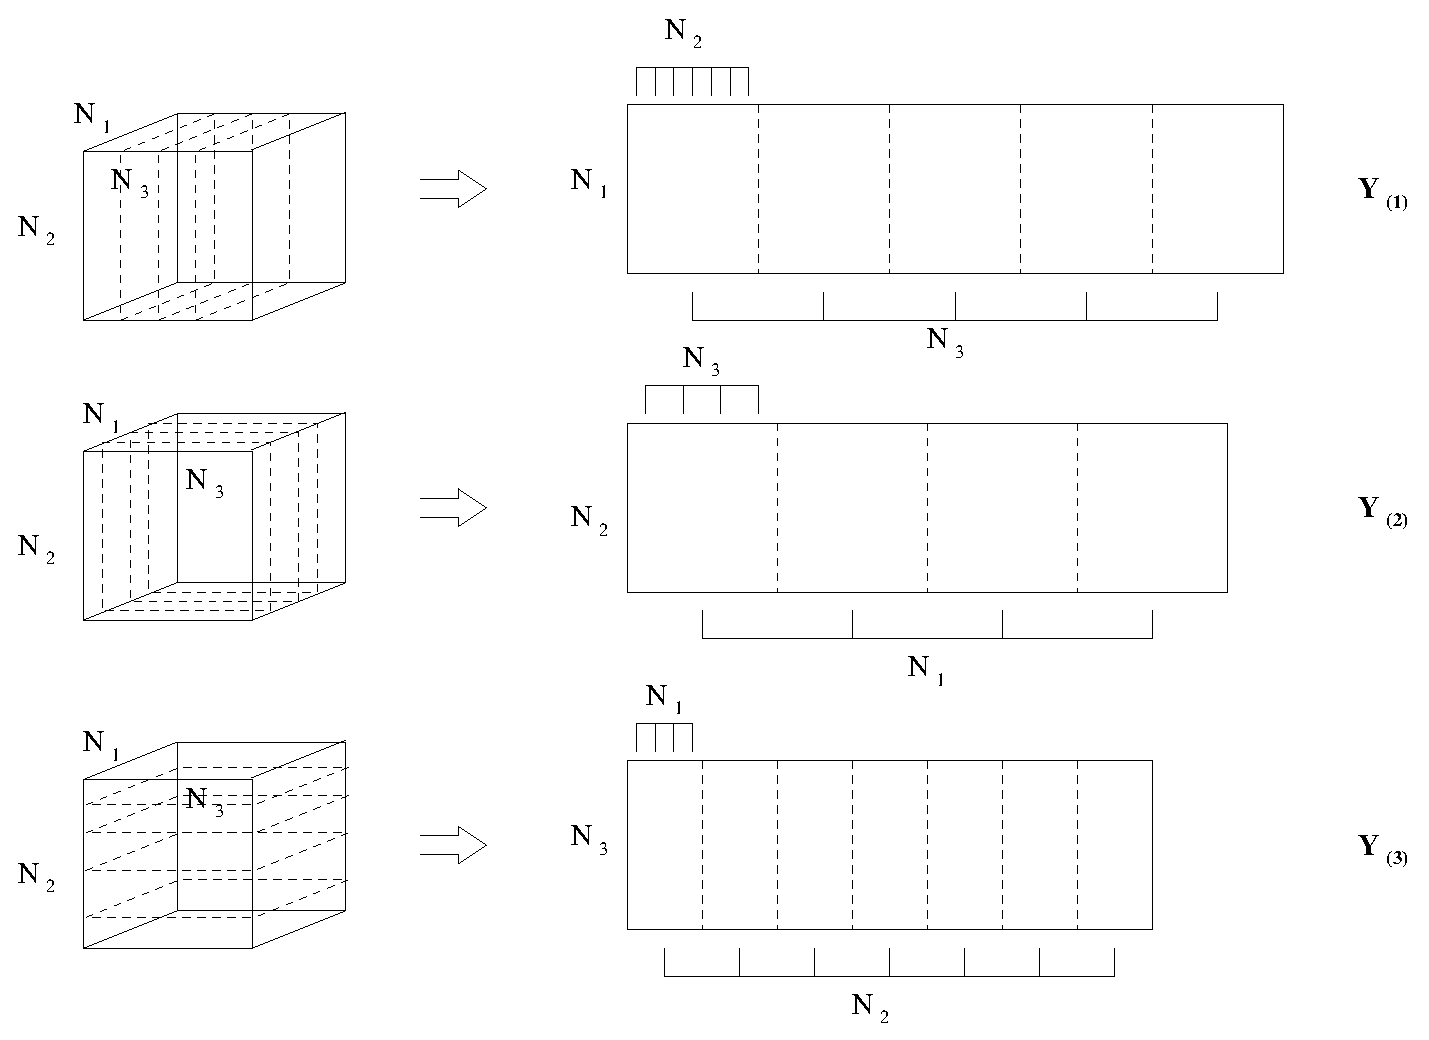
\includegraphics[width=0.7\linewidth,angle=0]{your_chapter_bibitem/fig1.eps}
\end{center}
\vspace{-4mm}
\caption{Your caption}
\label{fig:your_name_fig1}
\end{figure}
%

%
\begin{figure*}[htb]
\begin{center}
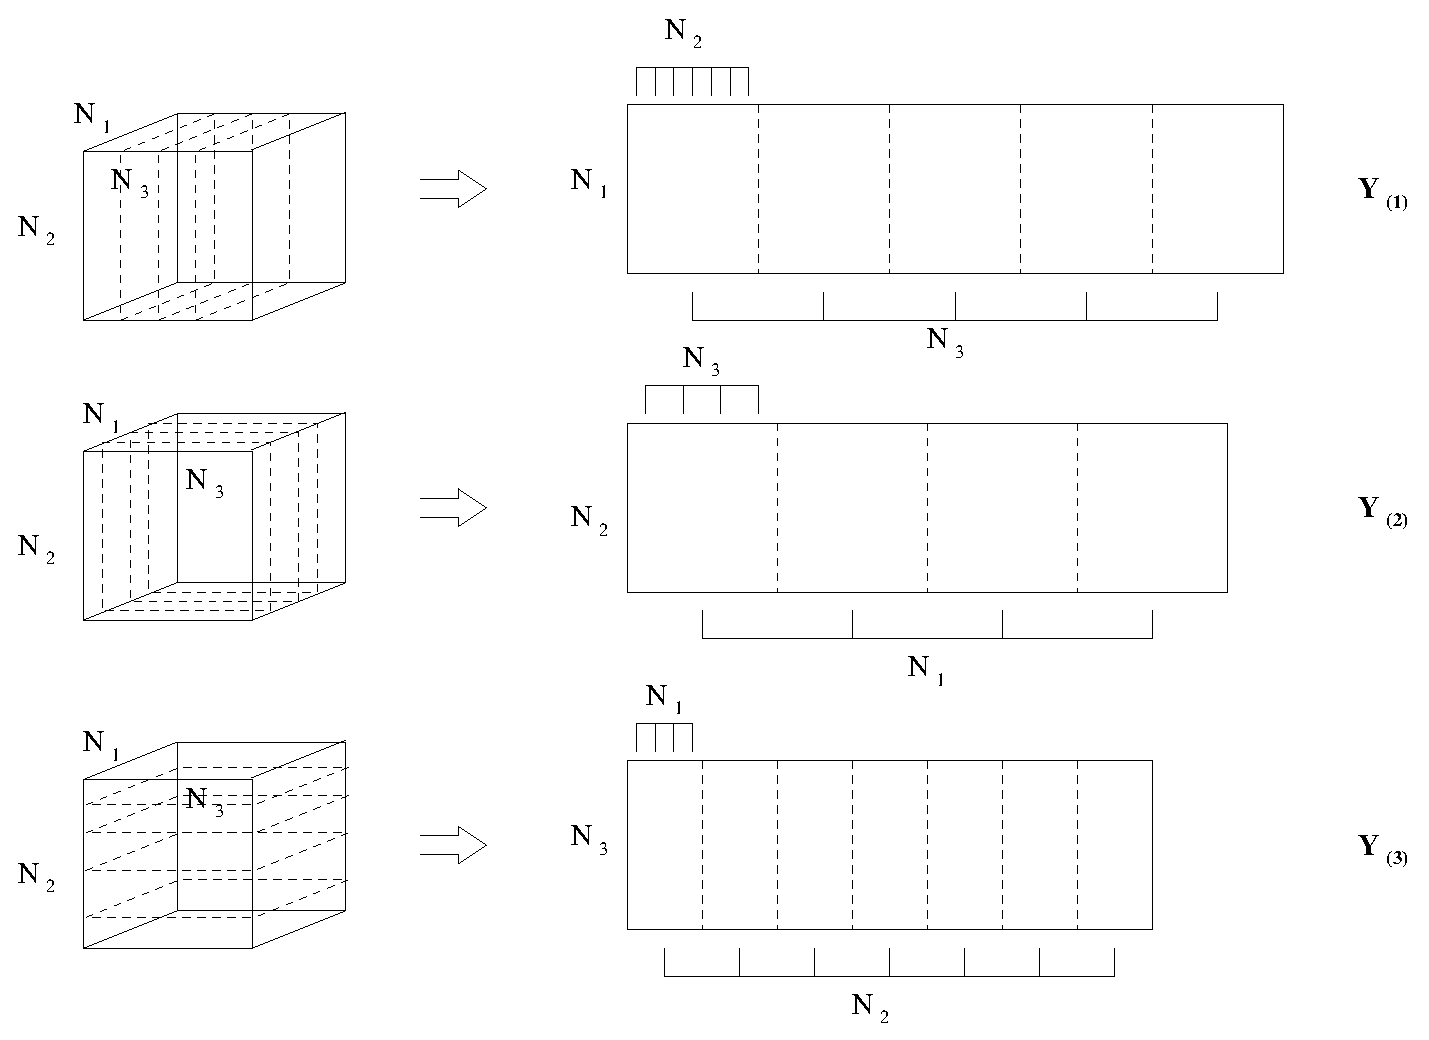
\includegraphics[width=0.7\linewidth,angle=0]{your_chapter_bibitem/fig1.eps}
\end{center}
\vspace{-4mm}
\caption{Your caption}
\label{fig:your_name_fig2}
\end{figure*}
%


%
\section{Acknowledgments}
%
The author would like to thank the sponsors of the Microseismic Industry Consortium for financial support.
%

\begin{thebibliography}{}
\itemsep0pt

\bibitem[Van~der Baan, 2008]{VanderBaan2008}
Van~der Baan, M., 2008, {Time-varying wavelet estimation and deconvolution by
  kurtosis maximization}: Geophysics, {\bf 73}, no. 2, V11-V18.

\end{thebibliography}

 
\cleardoublepage
%-------------------------------------------------------------------------------
% Definitions
%-------------------------------------------------------------------------------
% here we define authors and titles
%
\providecommand{\theauthorsfull}{Anton Biryukov, Jan Dettmer and David Eaton} %full list of authors - eg Mirko van der Baan and David Eaton
\providecommand{\theauthorsshort}{Biryukov et al.} %short list of authors (max 40 characters} - eg Van der Baan and Eaton or Van der Baan et al.
\providecommand{\thetitlefull}{Event origin depth uncertainty - steps towards estimation and mitigation using waveform similarity}
\providecommand{\thetitleshort}{Location depth error mitigation} % max 40 characters
%-------------------------------------------------------------------------------
% REPORT SECTION
%-------------------------------------------------------------------------------

%\chapter[\theauthorsshort: \thetitlefull]{\thetitlefull \\ \vbox{}
%\vbox{}
%{\small\em 
% place address here
%${}^a$ Department of Geoscience, University of Calgary, Calgary, AB, T2N 1N4, Canada.  E: anton.biryukov@ucalgary.ca \\[-10pt]
%}} % don't remove!
%

\chapter[\theauthorsshort: \thetitlefull]{\thetitlefull \\ \vbox{}
{\LARGE\em  Anton Biryukov, Jan Dettmer and David Eaton}\\ %Replace with your own list of authors
\vbox{}
{\small\em 
% place address here
${}^a$ Department of Geoscience, University of Calgary, Calgary, AB, T2N 1N4, Canada.  E: anton.biryukov@ucalgary.ca \\[-10pt]
%${}^b$ Dept. of Physics, Univ. of Alberta, Edmonton, AB, T6G 2G7, Canada.  E: Mirko.vanderBaan@ualberta.ca
}} % don't remove!



\rhead[Microseismic Industry Consortium Vol. \thereportvolume\ -- Chapter \thechapter]{\em \thetitleshort}
\lhead[\theauthorsshort]{Microseismic Industry Consortium Vol. \thereportvolume\ -- Chapter \thechapter}

%
\section*{Summary}
%
The induced seismicity event localization using inverse kinematic algorithms is still a problem requiring special attention. Often a catalog of events detected and located using limited on-surface instrumentation lacks the precision of origin depth. Such errors can hinder the interpretation of activated zones using seismicity as a proxy.

The location constraints are affected by the inaccuracy of the velocity model, limited acquisition geometry and the assumptions inherited by the location algorithm, among other factors. The issue becomes even more aggravated when only surface arrays are employed, where the geometry strongly favors the accuracy of epicentral location as opposed to depth location. The reported depth errors are sometimes comparable to a formation thickness or even the origin depth itself.

The locations are often done using the phase first breaks only. Finding additional features of the seismic signal that could be informative of its origin can be a first step towards constraining the depth uncertainty. Therefore, the purpose of this study was two-fold. First, we characterized the uncertainty in the event origin due to the inaccuracy in the effective velocity model. Using Monte-Carlo simulations for a given velocity model uncertainty, the event origin and the receiver array, we simulate the traveltimes at the stations and then relocate the event using the baseline velocity model. We show that the presence of a low velocity zone (LVZ) can cause the non-uniqueness and a spread of the solution over a large depth range. This spread was found to depend on the scale of the velocity model uncertainty, whereas the epicenter of the event showed low sensitivity to velocity model perturbations. Subsequently, a wave number integration method was utilized to simulate the synthetic seismograms from the synthetic earthquakes spanning the depth range of 2-5km, covering LVZ. For a fixed focal mechanism and frequency content, we numerically generate a bank of waveforms corresponding to the virtual events with known locations. The bank is then divided into a training, cross-validation and test parts. A set of classifiers is trained to predict the event location with respect to LVZ based on arrival times and statistical features of the signal waveforms. We demonstrate that adding several features of the signal, descriptive of its origin can improve the location depth constraint, as opposed to using arrival times only as predictor variables.
%
\section{Introduction}
The earthquake localization on a regional scale using inverse kinematic algorithms is still a problem requiring special attention. The on-surface seismic networks for monitoring induced seismicity provide a sufficient location accuracy for the earthquake hypocenter, but often offer very limited resolution in depth (\cite{eisner_uncertainties_2009}). The precision of the earthquake location is affected by many factors, including the lack of knowledge in the velocity model, limited acquisition geometry and the assumptions inherited by the location algorithm. For computational convenience and due to the lack of information, the velocity model used for location is often parametrized as a function of depth only. This type of parametrization leads to a laterally homogeneous model, which is sometimes referred to as a 1D or a ``layered cake'' model. In some cases such an approximation is a very strong assumption, and it is important to consider several different possible 1D structures to test the sensitivity of the location to errors in the velocity model.

The sparsely distributed on-surface instrumentation and insufficient azimuthal or vertical coverage can aggravate the location uncertainty due to the limited direction of the ray-paths it is able to receive. In contrast to that, the downhole arrays are able to provide a stronger constraint on the depth as they record the rays propagating predominantly within the layer (\cite{eisner_comparison_2010}). As a result, in the absence of downhole observations, the reported uncertainty of the depth location using on-surface array only may be comparable to the origin depth value itself, such that the location of the event becomes untrustworthy to the analyst. 

On the other hand, the sophistication of the location algorithms may not permit resolving this issue. In fact, in the daily industry practice the event origins are often derived based on the deterministic methods that use only 2 characteristic points (P- and S-wave arrivals) per sensor per event. The information transmitted by the event is obviously not limited to two-points only, and therefore should not be discarded when the location is performed.

Improving event location using additional information from the event signal is a complex problem. Therefore, it is important to disassemble this problem into tractable smaller sub-problems. One of sub-tasks is finding informative features of the seismic signal that could help better constrain the location. 


We start with a rigorous study of the effect of the uncertainty in the velocity model on the P- and S-wave travel time error. The ray-tracing method is employed to predict the time of the arrivals for the two phases at station location. The Monte-Carlo simulation is then performed with varying velocity model to estimate the mean and standard deviation of the arrival time. These values are consequently used as a proxy for an event's P- and S-wave arrival time uncertainties. Using non-linear location methods (\cite{lomax_precise_2001}), the arrival times from the Monte-Carlo simulations can be translated into spatial uncertainties and thus give an error estimate due to uncertainty in the velocity model, given an event location.


Subsequently, a wave number integration method is utilized to simulate the synthetic seismograms from the synthetic earthquakes spanning the depth range of 2-5km. A set of characteristic functions is applied to the resultant synthetic traces in order to extract the features describing the origin of the signal. Subsequently, a classification of the event location is carried out on two separate feature sets: (i) arrival times only and (ii) arrival times bundled with the signal features. With this comparison we highlight that even for such a simple task the travel time data may be insufficient to constrain the origin of the event due to the velocity model accuracy. However, adding the waveform features has a potential to constrain the origin depth, positively affect the location quality in terms of prediction accuracy, and can be a promising direction of further research.

\section{Methods}
%
This section provides a brief overview of the methods employed in this study. As our first goal was to estimate of the uncertainty in origin depth, we start with a description of the travel time calculation method based on the ray theory, followed by the summary of the event location algorithm employing the predicted travel times. Our second goal was to implement a classifier capable of determining the signal origin based on the arrival times and signal features. Therefore, this section also provides the workflow for preparing the feature set from the event waveforms and training such a classifier on the available data.

\subsection{Generalized workflow}
This report is particularly focused on estimating the depth error due to the velocity model uncertainty. That is, we want to evaluate the jitter in the hypocenter location due to inaccuracy in the approximation of the true velocity model as a 1D layered cake model derived from $V_{p}$ and $V_{s}$ logs. Specifically, we would like to simulate the travel times from many virtual events with a fixed origin but variable velocity model. These travel times are then used for relocating the events, that should potentially result in a cloud centered at the origin. The spatial dimensions and the shape of the cloud can give a quantitative insight into how sufficient the 1D velocity model assumption might be for a particular region and acquisition geometry.

Therefore, the general workflow can be summarized in several key steps as follows:
\begin{itemize}
 \item determine the background (expected) velocity model from the sonic logs,
 \item carry out many (9000) Monte-Carlo (MC) simulations for the travel time sets in a perturbed velocity model for an event with a fixed origin,
 \item treating each travel times set independently, locate the event corresponding to the set using background velocity model,
 \item analyze the PDF of the obtained distribution.
\end{itemize}



\subsection{Monte - Carlo travel time simulations}
 As no anisotropy or 2D elastic profile information was available, the baseline velocity model was approximated as a 1D laterally homogeneous layered medium. The elastic parameters for the layers were derived from the sonic wellbore logs. The velocity uncertainty in this study is modeled through applying a random normal perturbation of $V_{p}$ and $V_{s}$ within a layer, while keeping the thickness of the layers constant. The standard deviation of the perturbation is a fraction of the velocity value within the layer. An example of the velocity profile distribution with the 6\% standard deviation is shown in Figure \ref{fig:vpvs}, with color showing the probability density function (PDF) for the values of $V_{p}$ and $V_{s}$ within the layer.

\begin{figure}[htb]
\begin{center}
\includegraphics[width=0.7\linewidth,angle=0]{./AntonBiryukov_bibtex/VpVs.png}
\end{center}
\vspace{-4mm}
\caption{An example of the distribution of velocity profile used in the MC simulations. The color represents the values of PDF of the velocity distribution. Note the limited variation of the layer above LVZ due to the creation of the shadow zone.}
\label{fig:vpvs}
\end{figure}

Currently, there exist various methods for computing synthetic seismograms (\citet{kennett_seismic_2001}, \citet{chapman_fundamentals_2004}). In the case of a 1D layered medium the classic seismic ray theory can produce an exact solution for the phase travel times assuming high frequency content of the signal, at a very low computational cost. Therefore, a Python-based implementation of a ray tracing method (Pyrocko-Cake by S. Heimann, available at http://emolch.github.io/pyrocko/) was chosen as a best fit-for-purpose method. Pyrocko-Cake allows robust obtaining travel times for a custom phase (e.g. direct P ($t_{p}$) and a direct S ($t_{s}$)) between a specified source and a receiver pair.


It is important to notice that for some of the MC realizations the travel times for all four stations were not available due to the strong velocity contrast created at 3200 meter depth. The presence of the contrast caused significant reflection leading to shadowing of the direct P-phase at larger offsets, and as such the realizations were discarded from the analysis. That effect is visible in the Figure \ref{fig:vpvs} by a limited accepted variation of $V_{p}$ within the layer at 2500 - 3200 meters depth.

\subsection{Event origin location} % Mention somewhere in discussion / intro the comparison between Linearized and DIRECT SEARCH!!!!!!!!!!!!!!!!!!!!!
In the case of a limited recording geometry and a velocity model with sharp horizontal interfaces, a probabilistic direct global-search procedure was shown to outperform the linearized location methods and adequately determine the complete location PDF of the event, converging to a global maximum (\citet{lomax_earthquake_2009}). Therefore, we opted for employing the probabilistic, non-linear, global-search earthquake location algorithm implemented in the NonLinLoc software \cite{lomax_precise_2001}. NonLinLoc has gained its popularity due to simple logic and easy-to-use interface, its robustness and currently is transitioning to become a standard for regional and global earthquake location.

The NonLinLoc program outputs a misfit function, an estimate of the posterior PDF for the spatial hypocenter location, and other results using stochastic, Metropolis-Gibbs sampling approach. The errors in the phase time picks and in the forward problem (travel-time calculation) are assumed to be Gaussian. This assumption allows for the analytic calculation of a maximum likelihood origin time given the observed arrival times and the calculated travel times between the observing stations and a point in space. To achieve efficiency for complicated, 3D models, the travel-times between each station and all nodes of the spatial grid are calculated once and then stored on disk as travel-time grid files.

The algorithm searches the grids to find the best-fitting set of travel-times that would approximate the observed travel times for an event. In these simulations we use only local four stations, and utilize both P and S picks for each station, a total of 8 travel times. The spatial volume used for grid-search or Metropolis-Gibbs location must be fully contained within the 3D travel-time grids. This limits the largest station distance that can be used for location since the 3D travel-time computation and the size of the output time-grid files grow rapidly with grid dimension. In our case however, the zone of interest is well constrained within the station array, thus satisfying the NonLinLoc requirements.

\subsection{Synthetic waveform modeling}
The synthetic waveforms used for event origin classification were produced using the wavenumber integration method implemented in CPS suite (\cite{herrmann_computer_2013}). For the particular case of 1D layered homogeneous media, CPS allows one to obtain the full waveforms from the source much quicker than 2D Finite Difference methods commonly used for similar purposes.

For each of the source-receiver pairs simulated in the model we generate a database of Green's functions. The Green's functions are then convolved with the source wavelet of the given dominant frequency $f=2.5$ Hz and a given moment tensor $M_{i,j}$ corresponding to a pure explosive source (identity matrix). To achieve variability in the signal waveforms and mimic realistic amplitude uncertainty, the moment tensor was perturbed with a Gaussian noise:
\begin{equation}
 M_{i,j} = 1 + \sigma_{m},
\end{equation}
where $\sigma_{m} = 0.1$ is the standard deviation of the perturbation. The uncertainty of the velocity model is taken into account by applying a random shift in time to the waveforms, and perturbing $t_{p},t_{s}$ with the standard deviation derived from the Monte-Carlo simulations described above. Subsequently, a set of statistical and deterministic features is extracted from the waveforms in order to bring more information about the origin of the signal. Specifically, we want to describe the signal properties that are expected to change due to the relative position of the origin with respect to the strong reflector. Prior to the feature extraction, the signals are all normalized to a unit amplitude. We then obtained the envelope of the signal on the vertical channel using Hilbert transform and chose the following features as the proxy:
\begin{itemize}
 \item kurtosis of the signal envelope - to show the peaked-ness of the signal and discern between signals with strong and weak multiple reflections,
 \item mean value of the envelope,
 \item standard deviation of the envelope - to show the variability in the envelope,
 \item area under the envelope,
 \item the ratio of the signal energy contained between $t_{p}$ and $t_{s}$ with respect to the whole trace
 \item number of zero-crossings of the envelope derivative - to count the number of local extrema of the envelope
\end{itemize}

The procedure of modeling and feature extraction is then repeated over the set of values for the moment tensor $M_{i,j}$ and locations covering the range of 2000-5000 meters, thus creating an large dataset for the subsequent classification. It is important to notice that the list of features is by no means exhaustive and can be altered and augmented if necessary. The choice of the most representative features for the particular problem is a complicated task by itself and is therefore out of scope for this study. Our main goal was to show whether adding easily available information can positively affect the location accuracy judged by the classification score or not.
\subsection{Signal classification}
\begin{figure*}[htb]
\begin{center}
\includegraphics[width=0.85\linewidth,angle=0]{./AntonBiryukov_bibtex/classes.png}
\end{center}
\vspace{-4mm}
\caption{An illustration of the signal classification concept. The signals originating from the locations on the grid (a) are then transformed into a feature space and labeled by the class containing the event origin.}
\label{fig:classes}
\end{figure*}
The concept of the classification is briefly illustrated in Figure \ref{fig:classes}. The zone of interest is first meshed into a grid, where each node can host virtual sources. The signal from an event originating at a node is transformed into the feature space by selecting representative properties of the signal and is labeled according to the location of the grid. After transformation, the signal database obtained from the synthetic waveform modeling has been divided into 3 classes by the origin depth of the event: (i) above LVZ, (ii) within LVZ, and (iii) below LVZ. The positions were then marked according to their relative location with respect to the LVZ as demonstrated in Figure \ref{fig:foxcreek_classes}. For each position of the virtual source 150 simulations with different values of $M_{i,j}$ were carried out. The database was later split into the training (70\% of the total data) and the test datasets (30\% of the total). 

\begin{figure}[b!]
\begin{center}
\includegraphics[width=0.85\linewidth,angle=0]{./AntonBiryukov_bibtex/figure_foxcreek_classes.png}
\end{center}
\vspace{-4mm}
\caption{The relative virtual source-receiver locations for the classification experiment. The colorscale indicates which class an event belongs to.}
\label{fig:foxcreek_classes}
\end{figure}

A set of classification algorithms was trained on the training data in order to predict the focal depth of the event (its class) given a set of features of an event of interest from the test data. It is valuable to compare the performance of different rather simple classifiers on this problem before moving towards a more complex solution. Therefore, a comparison of prediction accuracy was done between a non-generalizing algorithm - K-nearest-neighbors (\cite{cover_nearest_1967}), and linear classifiers - logistic regression (\cite{jr_applied_2004}) and Support Vector Classifier (\cite{suykens_least_1999}). The comparison can help choose the more robust classification method for the future work, as well as identify the generalization character of the problem. The picked classifiers are easy to tune since the parametrization is done through one or two parameters, and as such serve as great candidates for a preliminary analysis. 

Python-based Scikit-Learn package was chosen as an implementation of the aforementioned algorithms. The fine-tuning of the internal algorithm parameters, e.g. regularization parameter $C$ for logistic regression and SVC, has been done through exhaustive grid search over the parameter space. The purpose of fine-tuning is to find the optimal set of parameters producing the highest prediction accuracy on the test set.

The output results of the classification can be interpreted in several ways. Here we limit ourselves to the interpretation of the confusion matrix of the test set. The elements of the confusion matrix $c_{i,j}$ show the number of observations from class $i$ predicted into class $j$. As a result, non-zero off-diagonal elements indicate the number of mislabeled observations, whereas the diagonal elements indicate the number of correctly predicted observations.
\section{Results}
In this section we first demonstrate the estimated depth and origin location uncertainties as obtained from MC simulations, followed by the summary of classification accuracy using several different classifiers.
\subsection{Origin uncertainty estimation}
The origin depth uncertainty was estimated for the 1\% and 6\% velocity perturbation. For both simulations the true location of the event was $(X,Y,Z) = (4000,6000,3910)$, which corresponds to the location of the main shock of January 2015 Fox Creek swarm. The location centroids of MC simulated events for the two models are shown in Figure \ref{fig:sigma1} and Figure \ref{fig:sigma6}, respectively. One may see that in both cases the X and Y coordinates of the event are centered at their true values. The depth of the event is centered 240 meters above the true focal depth in the case of 1\% model. In the 6\% model case the event depth shows a bi-modal distribution, with stronger mode centered 240 meters above the depth. The weaker mode, however tends to center around the true depth of the event. The standard deviation of the depth shows a noticeable increase as the velocity perturbation increases.
\begin{figure*}[htb]
\begin{center}
\includegraphics[width=0.8\linewidth,angle=0]{./AntonBiryukov_bibtex/Figure1_1pct.png}
\end{center}
\vspace{-4mm}
\caption{The results of the location of 1\% velocity perturbation Monte-Carlo simulated virtual events describing the true event at $(X,Y,Z) = (4000,6000,3910)$. The receivers are shown in black triangles, the virtual event centroids - in orange circles.}
\label{fig:sigma1}
\end{figure*}

\begin{figure*}[htb]
\begin{center}
\includegraphics[width=0.8\linewidth,angle=0]{./AntonBiryukov_bibtex/Figure1_6pct.png}
\end{center}
\vspace{-4mm}
\caption{The results of the location of 6\% velocity perturbation Monte-Carlo simulated virtual events describing the true event at $(X,Y,Z) = (4000,6000,3910)$. The receivers are shown in black triangles, the virtual event centroids - in orange circles.}
\label{fig:sigma6}
\end{figure*}

For the sake of comparison, the origin errors for the individual locations due to the traveltime pick uncertainty of 10 ms are shown in Figure \ref{fig:ind_error}. One may notice that the uncertainties due to the picking error are an order of magnitude smaller than those shown previously in Figure \ref{fig:sigma1} and Figure \ref{fig:sigma6}.

\begin{figure}[htb]
\begin{center}
\includegraphics[width=0.85\linewidth,angle=0]{./AntonBiryukov_bibtex/figure_inderr.png}
\end{center}
\vspace{-4mm}
\caption{The distribution of the origin uncertainties for individual virtual event locations. The scale of the errors are an order of magnitude lower than the uncertainty due to the unknown velocity model}
\label{fig:ind_error}
\end{figure}

\subsection{Signal origin classification results}
\begin{figure}[htb]
\begin{center}
\includegraphics[width=0.95\linewidth,angle=0]{./AntonBiryukov_bibtex/figure_map_a.png}
\end{center}
\vspace{-4mm}
\caption{The distribution of induced seismicity in Fox Creek area for the events of winter 2015. The central cluster modeled in this study is shown in cyan.}
\label{fig:map_clusters}
\end{figure}

The classification has been carried out on the database of 90 different earthquake origins distributed uniformly along the depth range of 2-5km and covering the area around the central Fox Creek seismicity cluster as shown in Figure \ref{fig:map_clusters}.
Here we limit ourselves to a three-class classification based on the proximity of the origin to the LVZ as indicated by the color of the event origin in Figure \ref{fig:foxcreek_classes}.
The classification has been carried out for two feature sets: (A) the travel times for P- and S-phases at each station (a total of 8 features) and (B) the features from A bundled with the signal features extracted from the vertical channels as described in Methods section. The confusion matrices for the optimally set-up classifiers are shown in Figure \ref{fig:confusion}. One may see that KNN being a non-generalized method shows a better performance compared to SVC and logistic regression for both feature sets (89\% vs 85\% and 86\% for A, and 98\% vs 95\% and 95\% for B, respectively). The linear classifiers, while exhibiting slightly lower accuracy, are easier to generalize for the future study and do not require storing the dataset in the memory for future application. Therefore, the loss in the accuracy might be motivated by the win in the general applicability, which makes both SVC and logistic regression good candidates for the future study. The accuracy values shown in Figure \ref{fig:confusion} suggest that the added features indeed carry valuable information about the event origin, and consistently contribute towards an increase of in average 10\% in the accuracy of the classification.



\begin{figure}[htb]
\begin{center}
\includegraphics[width=0.85\linewidth,angle=0]{./AntonBiryukov_bibtex/Figure_confusion.png}
\end{center}
\vspace{-4mm}
\caption{The summary of the classification done with KNN, logistic regression and SVC. The matrices show the proportion between the true and predicted labels on the test dataset.}
\label{fig:confusion}
\end{figure}

\section{Discussion}
% TO DISCUSSION
As noticed earlier in the Results section, the distribution of the origin depth in the Monte-Carlo simulations shows two distinct modes - 240 metes above the true origin and at a true origin depth. On one hand, this might be the consequence of the surface acquisition geometry resulting in predominantly near-vertical ray-paths at the surface layer, as opposed to the downhole arrays. On the other hand, it might be caused by the limited and only positive variation allowed for the layer above the LVZ due to the P phase shadowing for farther offset stations.


Due to its location with respect to the array, the central cluster is characterized with lower values of horizontal location error compared to other clusters (Figure \ref{fig:map_clusters}). However, as seen from the error distribution, the depth of the location is still poorly constrained for the central cluster and in some cases exceeds 500 m. Our results from the MC simulations suggest that an error in depth of this magnitude is quite realistic as it reasonably agrees with the predicted depth error for the event at approximately the cluster depth. Therefore, the 6\% velocity variation within the layers can be a fair estimate of effective velocity model uncertainty when analyzing the effects of the unknown velocity models.
It is also important to mention that the location was done here using the grid-search method. The estimates of the uncertainty are likely to change when a different method is used. The choice of the method here was motivated by the presence of a sharp velocity contrast, which often prevents the linearized methods from converging to a global minimum (\cite{lomax_earthquake_2009}).  


The background velocity model for this study was derived from the sonic log by dividing the measured interval into 6 layers and has not been calibrated. Such a division was based on one person's perception of averaging and layering. While for this particular region, setup and problem it might have been a satisfying approximation, it may not generalize well on the others. Therefore, more attention should be paid towards devising a robust method of velocity profile estimation. One of such methods could be the Reversible Jump Monte-Carlo Markov chain, that could treat the number of layers and values within as unknown and try to fit the step-like function that best explains the variation within the $V_{p}$ or $V_{s}$ log (\cite{sambridge_monte_2002},\cite{bodin_seismic_2009}).


It was somewhat expected to notice an increase in the accuracy of the origin depth prediction using the feature set with signal properties compared to the travel-time based prediction only. By calculating the properties of the signal related to the origin we expand the feature set and effectively add more information to learn from. Although we cannot provide a solid ground for choosing specific properties of the signal optimal for this problem, the choice of the particular features is not random, but rather logical. The energy transmitted by the signal, as well as the interbed reflection arrival times and amplitudes wound vary as the function of the event origin. Therefore, it is rational to experiment with the quantities of the signal sensitive to these phenomena. The classification approach demonstrated here is by no means exhaustive, and more work needs to be done in this potentially promising topic.


Given the low values of hypocenter uncertainties, a possible continuation of the work could be towards discretization the depth range and running an N-class classification, where N is the number of classes that would represent possible zones of signal clustering. Alternative route could be relating the signal waveforms to the physics that caused it, e.g. classification between natural earthquakes and mining blasts.


Finally, the long-term goal of the study is to apply the classification approach to the real data, and combine the real and synthetic datasets together to form a learning database. The success of this combination is based on many factors, including, but not limited to similarity of the synthetics to real data in the feature space, and the accuracy of the ground truth. Therefore, more research needs to be done in choosing the suitable set of signal features. The appropriate feature space would be the one where the real and the synthetic transformed data would have a significant overlap, suggesting that one is likely to represent the other. Devising such a feature space seems challenging, and needs to be addressed in case the inference needs to be done based on very limited real data. The accuracy of the ground truth is also of paramount importance since the lack of it may lead to prediction of erroneous results due to learning from the erroneous data. However, unlike the previous problem, this issue seems tractable in the cases when both downhole and surface seismic data might be available.





\section{Conclusions}
The purpose of this study was two-fold. First we analyzed the effect of the unknown velocity model on the uncertainty of the event origin depth when located using on-surface arrays with limited coverage in Fox Creek area. Our results show that for 6\% uncertainty in the velocity model we may expect up to 800 m of the depth error after the location is performed. The hypocenter of the event shows close to no variation compared to the focal depth variation, as expected given the on-surface acquisition geometry with sufficient azimuthal coverage. The scale of the error implies that the centroid of the event might be placed in two different formations, which can hinder the interpretation and might lead to erroneous conclusions.

Second, we experimented with several classification methods to determine whether features extracted from the signal can improve the accuracy of our location in a simple framework. We analyzed and compared the results of the classification of the event origin position with respect to the LVZ using travel times only versus travel times and the signal properties extracted from the vertical channels. Our results indicate that in the case of limited acquisition geometry the waveform features can be helpful in improving the accuracy of the origin depth prediction. 

The rigorous analysis of the features that would perform optimal for this problem is challenging and was out of scope of this project. Nevertheless, this project should be treated as a first step towards adding quantitative information about the waveform of the signal towards the location algorithms.




\section{Acknowledgments}
%
The author would like to thank the sponsors of the Microseismic Industry Consortium for financial support.
%

% 
%\addcontentsline{toc}{section}{References}
\clearpage
\nocite{*}
\bibliographystyle{seg} 
\bibliography{./AntonBiryukov_bibtex/bibloSponsors.bib}  
\cleardoublepage
%
%\thispagestyle{empty}
\rhead[]{\em References}
\lhead[\em References]{}
%\addcontentsline{toc}{chapter}{References}
%\bibliographystyle{seg} 
%\bibliography{example} 
\end{document}
